% En este punto, se pide inspeccionar **tres** de sus mejores modelos encontrados hasta ahora de cada familia de modelos: la mejor configuración para el árbol de decisión, la mejor configuración para LDA y la mejor configuración para SVM. Para ello:

% 1. Graficar curvas de complejidad para cada modelo (excepto para LDA), variando la profundidad en el caso de árboles, y el hiperparámetro C en el caso de SVM. Diagnosticar cómo afectan al sesgo y a la varianza esos dos hiperparámetros.
% 2. Graficar curvas de aprendizaje para cada modelo. En base a estas curvas, sacar conclusiones sobre si los algoritmos parecen haber alcanzado su límite, o bien si aumentar la cantidad de datos debería ayudar.
% 3. Construir un modelo **RandomForest** con 200 árboles. Explorar para qué sirve el hiperparámetro max_features y cómo afecta a la performance del algoritmo mediante una curva de complejidad. Explicar por qué creen que se dieron los resultados obtenidos. Por último, graficar una curva de aprendizaje sobre los parámetros elegidos para determinar si sería útil o no conseguir más datos.

% **Atención**: Tener en cuenta que debemos seguir utilizando AUC ROC como métrica para estas curvas.

% Para cada método pueden incluir hasta una carilla de texto y los gráficos que considere relevantes.

Procedemos en esta sección a inspeccionar los mejores modelos encontrados para los clasificadores \textit{árboles de decisión}, \textit{LDA} y \textit{SVM}. En particular, buscamos entender su comportamiento al aumentar su complejidad (variando alguno de sus hiperparámentros), trazar sus curvas de aprendizaje, y sacar conclusiones sobre sus varianzas y sesgo. Por último, los compararemos con un clasificador de tipo \textit{random forest}.

\subsection{decision trees}
Para el mejor modelo obtenido en la Figura \ref{random_tree}, variamos la \textit{profundidad máxima} para graficar las curvas de complejidad observadas en la Figura \ref{decisionTreeComplexity}. En ella podemos apreciar que, a partir de los clasificadores de \textit{altura máxima} $> 7$, el modelo se acopla completamente a los datos de entrenamiento, generando un \textit{overfitting}. A su vez, sus respectivas performances en los datos de validación decrementan desde el mejor valor de $\textit{altura máxima} = 4$ hasta estabilizarse en las alturas mayores a 8. Esto podría indicar que el modelo ya separó todas las instancias en sus respectivas hojas, y dejó de cambiar sus reglas de corte. Podemos también apreciar que durante la búsqueda aleatoria de hiperparámentros la combinación con \textit{altura máxima} 4 no se habría probado, de otro modo hubiese aparecido como la mejor.  
\begin{figure}[!htbp]
    \centering
    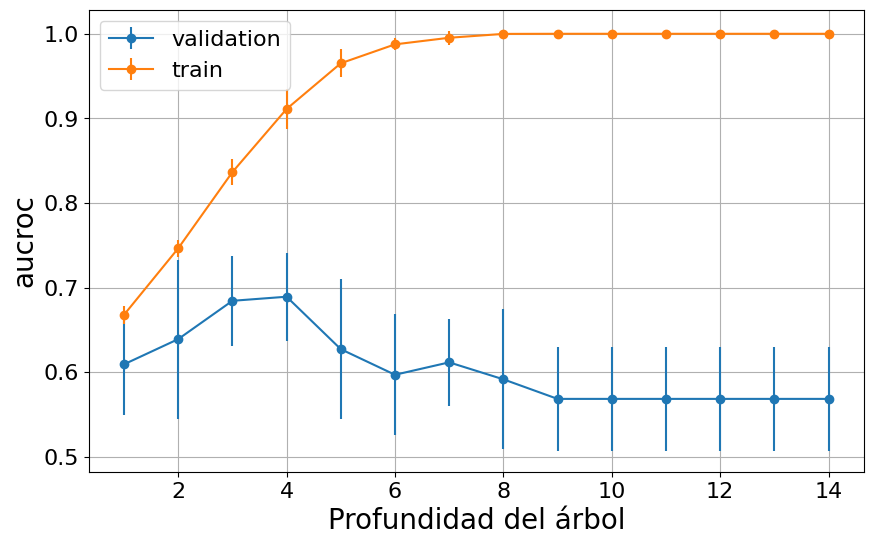
\includegraphics[width=0.75\textwidth]{/files/src/.media/decisionTreeComplexity.png}
    \caption{Curvas de complejidada para el clasificador \textit{decision tree}, mostrando la variación del AUC ROC en datos de entrenamiento y validación a medida que se aumenta su profundida máxima. Las lineas verticales denotan la varianza para cada valor del atributo.}
    \label{decisionTreeComplexity}
\end{figure}

Con respecto a la varianza, podemos observar que el rendimiento de los modelos varía considerablemente según el dataset utilizado en entrenamiento. Esto puede apreciarse en las barras de error\footnote{Estas provienen de las mediciones de AUC ROC para cada fold de validación.}, donde en algunos casos como para \textit{altura máxima} = 2 y 5, hubo una diferencia de performance en más de un $10\%$. A su vez, puede verse cómo se van separando ambas curvas a medida que aumenta la profundidad máxima. Es decir, la performance del modelo en entrenamiento aumenta al hacer \textit{overfitting} mientras que en validación decrece. Esto muestra que la varianza del clasificador crece junto con la profundidad máxima, ya que el modelo se acopla cada vez más al dataset.

Por otro lado, todos los resultados del algoritmo en validación se encuentran con un AUC ROC por debajo de $0.75$, y con media aproximadamente en $0.6$, con lo cual parecería tener poca capacidad predictiva. En ese sentido, sin importar el valor del hiperparámentro parecería ser un algoritmo incapaz de acercarse a la distribución subyacente de los datos, produciendo \textit{underfitting} y presentando un sesgo alto.

% 2. Graficar curvas de aprendizaje para cada modelo. En base a estas curvas, sacar conclusiones sobre si los algoritmos parecen haber alcanzado su límite, o bien si aumentar la cantidad de datos debería ayudar.

Variando la cantidad de datos de entrenamiento en el rango $[30, n]$ con un step de $10$, siendo $n$ la cantidad total de instancias, obtuvimos las curvas de aprendizaje de la Figura \ref{decisionTreeLearning}. De ellas podemos observar que, con pocos datos ($< 150$ instancias), el modelo parecería funcionar igual, a veces hasta peor, que un clasificador aleatorio, con un AUC ROC en promediado rondando el $0.5$. Al aumentar la cantidad de datos, puede observarse como ambas curvas se van acercando entre si, para luego estabilizarse en los valores $0.85$ para el set de entrenamiento y $0.6$ para el de validación. Esto indica que el algoritmo, sin importar cuánto aumentemos el tamaño del set de entrenamiento, parecería haber encontrado su límite de aprendizaje.

\begin{figure}[!htbp]
    \centering
    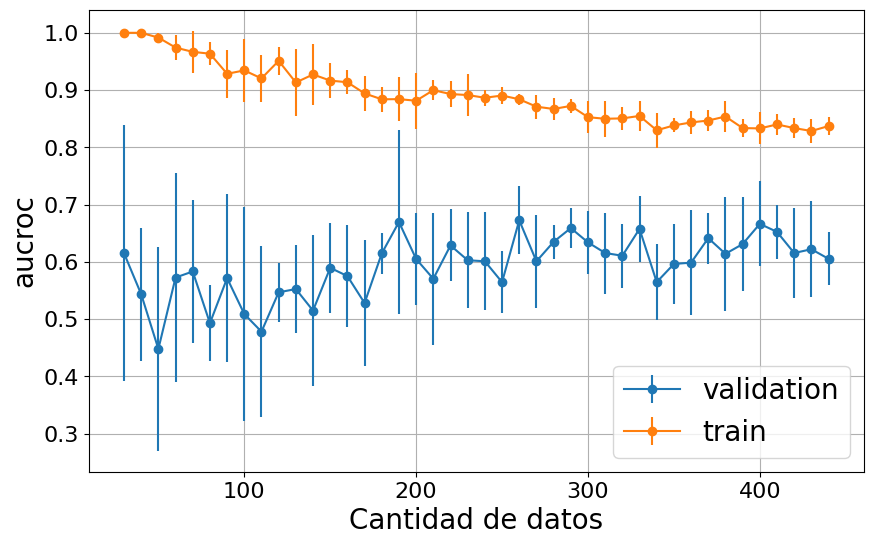
\includegraphics[width=0.75\textwidth]{/files/src/.media/decisionTreeLearning.png}
    \caption{Curvas de aprendizaje para el clasificador \textit{decision tree}, mostrando la variación del AUC ROC en datos de entrenamiento y validación a medida que se aumenta la cantidad de datos. Las lineas verticales denotan la varianza para cada tamaño de dataset.}
    \label{decisionTreeLearning}
\end{figure}


\subsection{SVM}
De la Figura  que los mejores hiperparámetros para este clasificador son:

\begin{itemize}
    \item \textit{Atributos Máximos} = 135.
    \item \textit{Criterio de Corte} = Entropía.
    \item \textit{Altura Máxima} = 3
\end{itemize}

Utilizamos este último para graficar las curvas de complejidad observadas en la Figura \ref{decisionTreeComplexity}. En ellas podemos apreciar que, respaldando los resultados de este clasificador en la sección anterior, obtenemos la mejor performance utilizando \textit{altura máxima} 3 y 4. Podemos intuir que durante la búsqueda aleatoria de hiperparámentros la combinación con \textit{altura máxima} 4 no se habría probado, de otro modo hubiese aparecido como la mejor.  

\begin{figure}[!htbp]
    \centering
    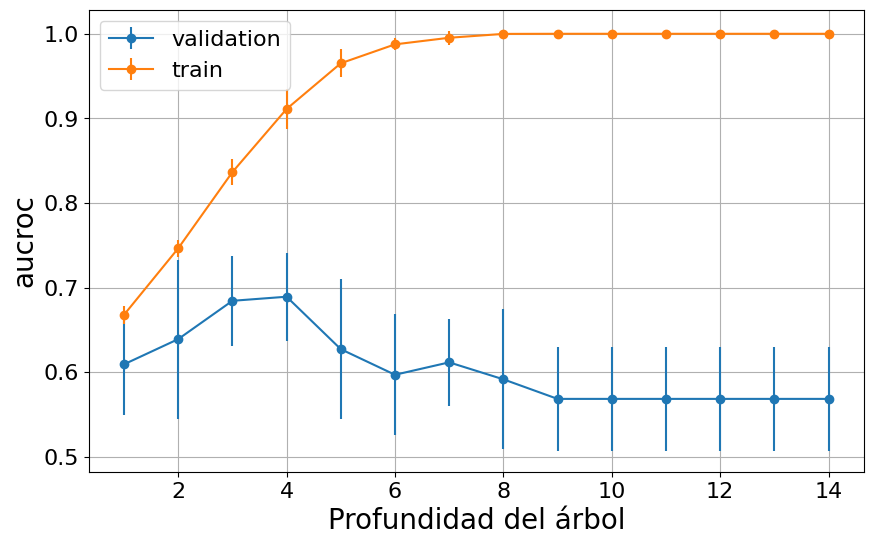
\includegraphics[width=0.75\textwidth]{/files/src/.media/decisionTreeComplexity.png}
    \caption{Curvas de complejidada para el clasificador \textit{decision tree}, mostrando la variación del AUC ROC en datos de entrenamiento y validación a medida que se aumenta su profundida máxima.}
    \label{SVMComplexity}
\end{figure}

A partir de los clasificadores de altura mayor a 7 se puede ver cómo el modelo se  acopla completamente a los datos de entrenamiento, generando un \textit{overfitting}. A su vez, sus respectivas performances en los datos de validación decrementan desde el mejor valor de \textit{altura máxima} = 4 hasta estabilizarse en las alturas mayores a 8. Esto podría indicar que el modelo ya separó todas las instancias en sus respectivas hojas, y dejó de cambiar sus reglas de corte. 

\subsection{random forest}
